\documentclass{article}
\usepackage[utf8]{inputenc}
\usepackage[spanish]{babel}
\usepackage{listings}
\usepackage{graphicx}
\graphicspath{ {images/} }
\usepackage{cite}
\begin{document}

\begin{titlepage}
    \begin{center}
        \vspace*{1cm}
            
        \Huge
        \textbf{PARCIAL 2}
            
        \vspace{0.5cm}
        \LARGE
        INFORME
            
        \vspace{1.5cm}
            
        \textbf{Michael Stiven Zapata Giraldo\\Brayan Steven Avila Marin}
            
        \vfill
            
        \vspace{0.8cm}
            
        \Large
        Despartamento de Ingeniería Electrónica y Telecomunicaciones\\
        Universidad de Antioquia\\
        Medellín\\
        Septiembre de 2021
            
    \end{center}
\end{titlepage}

\tableofcontents
\newpage
\section{ Analisis y diseño del problema }\label{intro}

Para este proyecto consideramos usar una matriz de leds 100x100 con tiras de 10 neopixels para la representación de las imagenes. Para programarla usaremos la librería Adafruit Neopixel. La conexión de la tira de leds es bastante sencilla, solo necesitaremos usar un solo pin del Arduino, y conectarlo al pin Din de la tira de leds, y en cada tira termina la conexion en la salida en el pin DO para en la siguiente conexion hacerla en la entrada de la siguiente tira y asi sucesivamente. Lo importante aca es tener en cuenta que cada led puede consumir hasta 60mA.

\section{Esquema}  
\begin{itemize}
\item Se define la cantidad de Led para hacer la matriz(100 leds con diez tiras)
\item Se utiliza una fuente externa de energia para la alimentacion de las tiras de leds desde el arduino
\item Se Implementa la clase dafruit Neopixel para crear efectos sobre las tiras de leds.

\end{itemize}


\begin{figure}[ht]
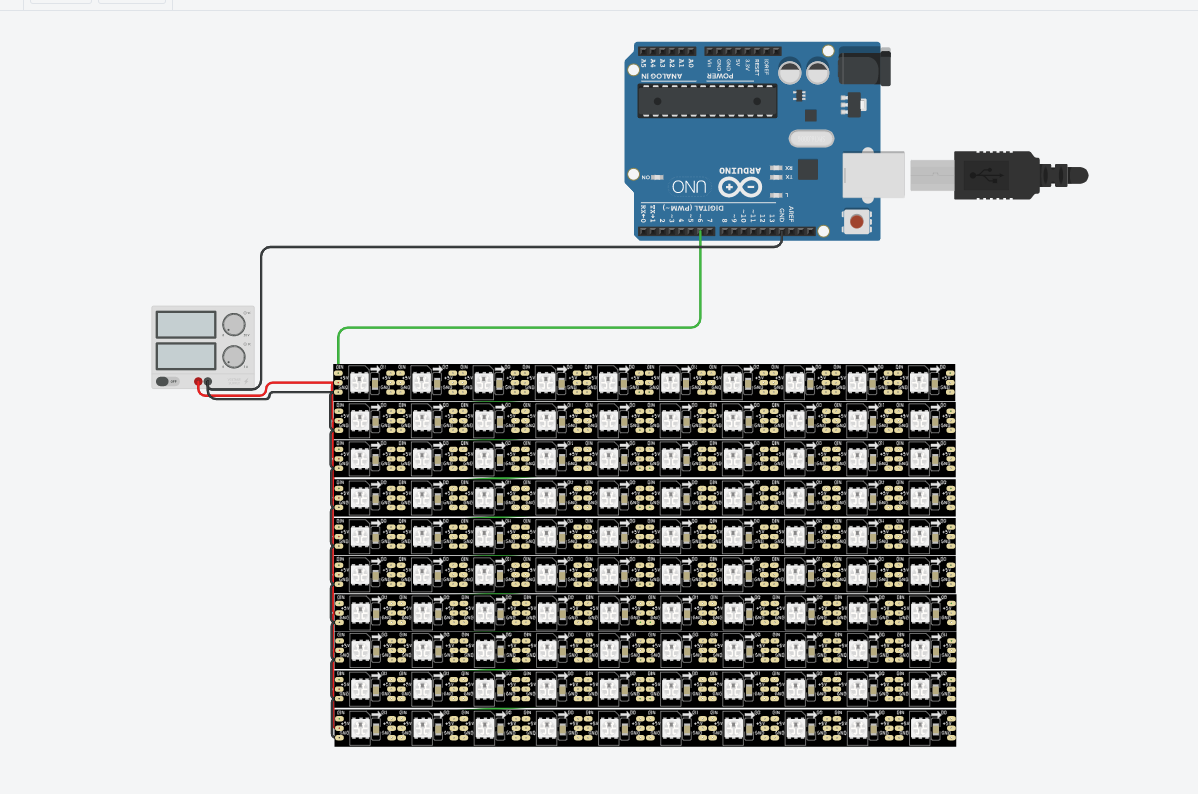
\includegraphics[width=12cm]{Esquema.PNG}
\centering
\caption{Esquema del montaje del circuito}
\label{fig:Montaje}
\end{figure}

\section{Algoritmo diseñado} 

\begin{enumerate}
    \item Leer la imagen en .JPG
    \item Convertir la imagen escribiendola como una matriz según la posición de sus pixeles
    \item Guardar dicha conversion en un archivo .txt
Para mostrar la imagen en la matriz de ledz
    \item Si la imagen es más grande que la matriz de leds
        \begin{itemize}
            \item Hacer submuestreo.
        \end{itemize}
    \item Si la imagen es mas pequeña que la matriz de leds
        \begin{itemize}
            \item Hacer sobremuestreo.
        \end{itemize}
    \item Mostrar el resultado encendiendo los leds para representar la imagen
\end{enumerate}

\section{Consideraciones a tener en cuenta en la implementación}
\begin{itemize}
\item Conexiones de las tiras de led: entrada por el pin DIN y salidas por el pin DO.
\item Establecer una fuente de energia o  fuente de voltaje de 5V/1A.
\item Utilizaremos la clase setPixelColor para apagar algunos leds y la clase show para actuaizar los leds

\end{itemize}

\end{document}
